\documentclass{article}

% Accepted workshop camera-ready.
\usepackage[dblblindworkshop,final]{neurips_2026}
\workshoptitle{SLMs for Agentic Systems, Paris, France, 2026}

\usepackage[utf8]{inputenc}
\usepackage[T1]{fontenc}
% hidelinks suppresses the default red link borders hyperref draws around every
% citation and cross-reference. The NeurIPS style does not load or configure
% hyperref, so this does not override any template setting. Links stay clickable.
\usepackage[hidelinks]{hyperref}
\hypersetup{
  pdftitle={How Should a Personal Agent Store Its Facts? Granularity, Compute, and Robustness in Parametric Memory},
  pdfauthor={Mahdi Ghodsi, Megha Sri Satya Sai Devineni, Chandra Shekhar Pandey}
}
\usepackage{url}
\usepackage{booktabs}
\usepackage{multirow}
\usepackage{amsfonts}
\usepackage{nicefrac}
\usepackage{microtype}
\usepackage{graphicx}
\usepackage{xcolor}

% All numeric macros are generated from the frozen results by
% paper2/make_tables.py. Nothing here is typed by hand.
% Generated by paper2/make_tables.py. Do not edit by hand.
\newcommand{\NPerArm}{200}
\newcommand{\NGradable}{181}
\newcommand{\NExcluded}{19}
\newcommand{\NAdaptersGated}{18}
\newcommand{\NAdaptersGatedAll}{148}
\newcommand{\GraderFloor}{0.0166}
\newcommand{\GTwentyQ}{0.602}
\newcommand{\GTwentyPQ}{0.541}
\newcommand{\GTwentyNad}{10}
\newcommand{\GTwentyTotMB}{283.2}
\newcommand{\GTwentyBuild}{7.06}
\newcommand{\GTwentyRet}{0.817}
\newcommand{\GFortyQ}{0.337}
\newcommand{\GFortyPQ}{0.359}
\newcommand{\GFortyNad}{5}
\newcommand{\GFortyTotMB}{141.6}
\newcommand{\GFortyBuild}{3.80}
\newcommand{\GFortyRet}{0.738}
\newcommand{\GHundredQ}{0.127}
\newcommand{\GHundredPQ}{0.171}
\newcommand{\GHundredNad}{2}
\newcommand{\GHundredTotMB}{56.6}
\newcommand{\GHundredBuild}{1.74}
\newcommand{\GHundredRet}{0.565}
\newcommand{\GTwoHundredQ}{0.116}
\newcommand{\GTwoHundredPQ}{0.144}
\newcommand{\GTwoHundredNad}{1}
\newcommand{\GTwoHundredTotMB}{28.3}
\newcommand{\GTwoHundredBuild}{1.14}
\newcommand{\GTwoHundredRet}{0.619}
\newcommand{\ResidentMB}{28.3}
\newcommand{\StorageRatio}{10}
\newcommand{\CurveLost}{91}
\newcommand{\CurveGained}{3}
\newcommand{\CurveP}{1.4\times10^{-23}}
\newcommand{\CurveNPaired}{181}
\newcommand{\StepTwentytoFortyLost}{58}
\newcommand{\StepTwentytoFortyGained}{10}
\newcommand{\StepTwentytoFortyP}{2.4\times10^{-9}}
\newcommand{\StepFortytoHundredLost}{41}
\newcommand{\StepFortytoHundredGained}{3}
\newcommand{\StepFortytoHundredP}{1.6\times10^{-9}}
\newcommand{\StepHundredtoTwoHundredLost}{9}
\newcommand{\StepHundredtoTwoHundredGained}{7}
\newcommand{\StepHundredtoTwoHundredP}{0.804}
\newcommand{\BaseQ}{0.050}
\newcommand{\BasePQ}{0.072}
\newcommand{\RetrQ}{0.729}
\newcommand{\RetrPQ}{0.613}
\newcommand{\SgdQ}{0.779}
\newcommand{\SgdPQ}{0.597}
\newcommand{\SgdRet}{0.660}
\newcommand{\SgdRetP}{3.8\times10^{-5}}
\newcommand{\GTwentyRetP}{0.061}
\newcommand{\RetrRet}{0.742}
\newcommand{\RetrRetP}{0.003}
\newcommand{\PairMinP}{0.31}
\newcommand{\SgdOptSteps}{249}
\newcommand{\SgdEpochs}{83}
\newcommand{\LoraAlpha}{32}
\newcommand{\LearningRate}{2\times10^{-4}}
\newcommand{\SgdFullQ}{0.906}
\newcommand{\SgdFullPQ}{0.547}
\newcommand{\NearBase}{0.119}
\newcommand{\NearGTwenty}{0.091}
\newcommand{\NearRetr}{0.068}
\newcommand{\PromptTokenRatio}{4.67}
\newcommand{\RetrTokens}{268.8}
\newcommand{\ParamTokens}{57.6}
\newcommand{\ExtraTokens}{211.2}
\newcommand{\SgdBuildTotal}{1731.5}
\newcommand{\SgdBuildPer}{173.2}
\newcommand{\DtwoLBuildPer}{0.706}
\newcommand{\BuildRatio}{245.3}
\newcommand{\RouterTopOne}{0.990}
\newcommand{\RouterMisGTwenty}{2}
\newcommand{\MaxRoutingDelta}{0.022}
\newcommand{\NondetChanged}{1}
\newcommand{\NondetGens}{56}
\newcommand{\NondetRouted}{200}
\newcommand{\SeedSteps}{249}
\newcommand{\SeedSeed}{42}
\newcommand{\SeedNAd}{18}
\newcommand{\ExpEpochs}{83}
\newcommand{\SeedGTwentyQ}{0.746}
\newcommand{\SeedGTwentyPQ}{0.597}
\newcommand{\ExpGTwentyQ}{0.773}
\newcommand{\ExpGTwentyPQ}{0.564}
\newcommand{\ExpGTwentySteps}{249}
\newcommand{\SeedGFortyQ}{0.702}
\newcommand{\SeedGFortyPQ}{0.470}
\newcommand{\ExpGFortyQ}{0.740}
\newcommand{\ExpGFortyPQ}{0.481}
\newcommand{\ExpGFortySteps}{415}
\newcommand{\SeedGHundredQ}{0.453}
\newcommand{\SeedGHundredPQ}{0.293}
\newcommand{\ExpGHundredQ}{0.762}
\newcommand{\ExpGHundredPQ}{0.403}
\newcommand{\ExpGHundredSteps}{1079}
\newcommand{\SeedGTwoHundredQ}{0.354}
\newcommand{\SeedGTwoHundredPQ}{0.298}
\newcommand{\ExpGTwoHundredQ}{0.757}
\newcommand{\ExpGTwoHundredPQ}{0.387}
\newcommand{\ExpGTwoHundredSteps}{2075}
\newcommand{\CompCurvePQP}{5.2\times10^{-19}}
\newcommand{\SeedCurveP}{8.4\times10^{-17}}
\newcommand{\SeedCurveLost}{77}
\newcommand{\SeedCurveGained}{6}
\newcommand{\SeedCurvePQP}{9.0\times10^{-11}}
\newcommand{\ExpCurveP}{0.766}
\newcommand{\ExpCurveLost}{24}
\newcommand{\ExpCurveGained}{21}
\newcommand{\ExpCurvePQP}{2.1\times10^{-5}}
\newcommand{\ExpCurvePQLost}{44}
\newcommand{\ExpCurvePQGained}{12}
\newcommand{\ExpQPMin}{0.42}
\newcommand{\ExpQLo}{0.740}
\newcommand{\ExpQHi}{0.773}
\newcommand{\ExpInteraction}{0.160}
\newcommand{\ExpInteractionCILo}{0.105}
\newcommand{\ExpInteractionCIHi}{0.212}
\newcommand{\ExpInteractionP}{0.0039}
\newcommand{\NAuthorClusters}{10}
\newcommand{\CompAuthorQP}{0.002}
\newcommand{\SeedAuthorQP}{0.002}
\newcommand{\ExpAuthorQP}{0.578}
\newcommand{\ExpAuthorPQP}{0.008}
\newcommand{\SeedBuildTwenty}{2027.6}
\newcommand{\ExpBuildTwenty}{1687.8}
\newcommand{\SeedBuildForty}{1188.2}
\newcommand{\ExpBuildForty}{1651.2}
\newcommand{\SeedBuildHundred}{458.0}
\newcommand{\ExpBuildHundred}{1562.4}
\newcommand{\SeedBuildTwoHundred}{243.4}
\newcommand{\ExpBuildTwoHundred}{1687.9}
\newcommand{\InitN}{19}
\newcommand{\InitQP}{1.00}
\newcommand{\InitPQP}{0.50}
\newcommand{\FullCtxQ}{0.862}
\newcommand{\FullCtxPQ}{0.834}
\newcommand{\FullCtxNHit}{156}
\newcommand{\FullCtxNGrad}{181}
\newcommand{\FullCtxQCILo}{0.804}
\newcommand{\FullCtxQCIHi}{0.905}
\newcommand{\FullCtxPQNHit}{151}
\newcommand{\FullCtxTokens}{7,567.6}
\newcommand{\FullCtxNFacts}{200}
\newcommand{\FullCtxLost}{12}
\newcommand{\FullCtxGained}{7}
\newcommand{\FullCtxRet}{0.923}
\newcommand{\FullCtxRetP}{0.359}
\newcommand{\FullCtxRatio}{131.4}
\newcommand{\FullCtxRatioRetr}{28.1}


% Default float parameters strand a lot of vertical space on pages that carry a
% figure or a table. Relaxing them lets text share those pages, which is what
% keeps the body inside the page limit.
\renewcommand{\topfraction}{0.92}
\renewcommand{\bottomfraction}{0.85}
\renewcommand{\textfraction}{0.08}
\renewcommand{\floatpagefraction}{0.80}
\setlength{\textfloatsep}{12pt plus 2pt minus 3pt}
\setlength{\floatsep}{10pt plus 2pt minus 2pt}
% Figure 1 and Table 1 show the same three regimes and are read together, and
% their combined height is well under \topfraction. The default \topnumber of 2
% is not the binding constraint; \totalnumber is, once a third float competes.
\setcounter{topnumber}{3}
\setcounter{totalnumber}{4}
\setlength{\intextsep}{10pt plus 2pt minus 2pt}

\title{How Should a Personal Agent Store Its Facts?\\
Granularity, Compute, and Robustness in Parametric Memory}

\author{%
  Mahdi Ghodsi \qquad Megha Sri Satya Sai Devineni \qquad
  Chandra Shekhar Pandey \\
  Advanced Micro Devices, Inc.
}

\begin{document}

\maketitle

\begin{abstract}
A personal language-model agent must keep a user's facts somewhere: as prompt
context at query time or encoded in adapter weights. When memory is partitioned,
both approaches require selection: one retrieves text into context and the other
activates a memory partition. The open design question is then not whether to
select but how finely to partition what is selected. We study this on a 4B instruction-tuned model over a fixed
\NPerArm{}-fact user memory, holding per-adapter rank constant at 16 and varying
the number of partitions across three adapter-construction regimes. Recall from
adapters compiled by a hypernetwork falls steeply as partitions coarsen, from \GTwentyQ{} at
20 facts per adapter to \GTwoHundredQ{} at \NPerArm{}, against a \BaseQ{} base
rate. Gradient-trained adapters given exactly \SeedSteps{} optimizer updates each
decline similarly (\SeedGTwentyQ{} to \SeedGTwoHundredQ{}, $p=\SeedCurveP{}$).
When instead every partition receives equal per-fact exposure at \ExpEpochs{}
epochs, original-question recall remains \ExpQLo{}--\ExpQHi{} without a monotonic
decline, while recall on paraphrased questions still deteriorates with coarser
partitions (\ExpGTwentyPQ{} to \ExpGTwoHundredPQ{}); the direct
question-form interaction is \ExpInteraction{} (author-clustered 95\% CI
[\ExpInteractionCILo{}, \ExpInteractionCIHi{}]). Granularity
therefore strongly affects parametric memory, but the relationship depends on the
construction regime and training exposure rather than on fixed adapter capacity
alone, and robustness and recall respond differently. We measure two in-context
points on the same items: among the five matched operating points,
placing all \NPerArm{} facts in every prompt reaches \FullCtxQ{} original and
\FullCtxPQ{} paraphrased recall at \FullCtxRatio{}$\times$ the prompt tokens of
the parametric arms per query, with top-5 retrieval intermediate on both accuracy
(\RetrQ{}) and cost (\PromptTokenRatio{}$\times$). No mechanism dominates every measured quality and
cost axis; we report what each one costs.
\end{abstract}

\section{Introduction}
\label{sec:intro}

An agent that runs on personal hardware has to remember its user: that your
daughter's recital is Thursday, that your build server is the one in the closet,
and several hundred other things no pretrained model was ever told. The
engineering question is where that knowledge lives.

The usual framing is a dichotomy: put the facts in the context window and
retrieve them, or bake them into the weights and dispense with retrieval. That
dichotomy misses the selection cost of partitioned parametric memory. A system
with one adapter per topic still selects: instead of retrieving text into the
prompt, it retrieves a \emph{memory partition} and activates it, so only the
delivery changes, tokens or weights. Once either representation is partitioned,
both approaches introduce a selection problem, and the interesting variable
becomes granularity: how much of a user's memory should one adapter hold? Coarse partitioning is cheap (one adapter, no routing, minimal
storage); fine partitioning can improve accuracy when construction work per
adapter is constrained, but costs bank storage, construction, and routing.

We fix a user memory of \NPerArm{} facts, fix per-adapter rank at 16, and vary how
many partitions the memory is split across: 20, 40, 100, and \NPerArm{} facts per
adapter, a bank of \GTwentyNad{} adapters down to a single monolithic one. Holding
per-adapter rank fixed might appear to make the sweep a pure capacity
measurement. Our results show that interpretation is too strong. How the adapters
are built matters as much as how the facts are divided: under a fixed per-adapter
budget of optimizer updates, recall on original questions falls steeply as
partitions coarsen, but when every partition instead receives equal per-fact
gradient exposure, that decline is not observed. What does survive equalizing
exposure is the paraphrase penalty (Figure~\ref{fig:granularity}). We then price
these organizations against what they cost, and against two in-context
alternatives on identical items: top-5 retrieval, and placing the entire
\NPerArm{}-fact memory in every prompt.

Our contributions:
\begin{itemize}
  \item \textbf{A controlled granularity $\times$ construction-budget study.} A
        four-point 20/40/100/\NPerArm{} facts-per-adapter sweep over one fixed
        \NPerArm{}-fact memory at fixed per-adapter rank, in three construction
        regimes (compiled, gradient at a fixed budget of \SeedSteps{} optimizer
        updates, and gradient at fixed per-fact exposure), with paired item-level
        tests in each (\S\ref{sec:curve}).
  \item \textbf{A separation of original-form recall from robustness.} Under
        equal per-fact exposure, the resolved coarse-granularity penalty on
        original-question recall is no longer observed, while the paraphrase
        penalty remains in every regime we measured (\S\ref{sec:curve}).
  \item \textbf{The systems accounting.} Five operating points on the same
        items, full context, top-5 retrieval, compiled and gradient adapters,
        and the memoryless base, priced against construction time, bank storage
        (\GTwoHundredTotMB{}--\GTwentyTotMB{}\,MB for the same facts), routing,
        and prompt tokens per query (\S\ref{sec:cost}, \S\ref{sec:operating}).
\end{itemize}

\section{Related work}
\label{sec:related}

Several prior works motivate partitioned adapter memory; we claim no priority for
the architecture itself. We hold per-adapter rank constant and vary the number of
partitions, but construction regime and exposure change how that sweep reads, so
it is not on its own a capacity measurement.

\paragraph{Capacity of a single adapter.} \citet{loramem} sweep data volume at
fixed rank and report a rank-dependent saturation point beyond which
``performance degrades sharply''; \citet{dataquality} internalizes 1--99 documents
and confirms ``a capacity trend (rank must grow with corpus size).'' Both vary
rank along their ladder or hold the adapter count at one; our axis is the number
of partitions with per-adapter rank held constant. \citet{adapterbits} find
1.7--2.75 bits per parameter and that placement matters more than count, which
motivates our MLP-side target module; \citet{memorylaw} fit a power law in rank
and sequence length, measuring loss not free-form recall, and
\citet{knowledgecapacity} establish the pretraining-scale analogue.

\paragraph{Partitioned and routed adapter memory.} \citet{loramem} also include a
partition arm, under the constraint that is the crucial difference from ours:
configurations are compared ``under an identical parameter budget,'' one rank-32
module against eight rank-4, so per-adapter capacity \emph{shrinks} as they
partition. We hold it fixed and let total storage grow, the constraint a
deployment faces when adapters are a fixed served artifact. \citet{d2a} already
build per-atom micro-adapters with a query router, so we claim no architectural
priority; their rank is fixed at 8, the atom count $K$ is a training curriculum
with inference fixed at $K=8$, and they name the granularity axis as future work.
\citet{cdlmm} distill each context into its own adapter and report that
``accumulating contexts weakens an adapter's ability to preserve context-specific
knowledge,'' but their cumulative baseline updates sequentially, confounding
forgetting with holding more content; ours are independent.

\paragraph{Compiling context into weights.} \citet{d2l} train a hypernetwork
converting a document into a LoRA in one forward pass, our compiled-memory
generator; their rank ablation holds content fixed while varying capacity, the
inverse of our sweep. \citet{cartridges} sweep cartridge size at a fixed corpus
and find LoRA scales poorly to large cartridges relative to prefix tuning; corpus
size is never varied. \citet{packlora} vary the number of injected facts but
measure damage to \emph{pre-existing} knowledge rather than recall of the injected
facts.

\paragraph{Personal memory.} \citet{oppu} attach a per-user parametric module
and find parametric and non-parametric memory complementary rather than
substitutable. \citet{substrate} and \citet{engram} argue that style and factual
recall respond oppositely to weight edits; we take that substrate split as given
and ask how to organize the factual half. We adopt the small-language-model
definition of \citet{slm}: a model below roughly 10B parameters fitting on a
consumer device.

\section{Experimental design}
\label{sec:design}

\paragraph{Setting and data.} A single user with \NPerArm{} personal facts, served
by one shared 4B base model small enough to run on hardware the user controls. The
facts are TOFU~\citep{tofu}, config \texttt{forget10\_perturbed}, fictitious author
biographies designed to avoid overlap with real-world factual knowledge. We do not
assume zero pretraining exposure, since TOFU predates the base model; the base arm
is the empirical check, and its \BaseQ{} recall indicates little of the evaluated
information is recoverable without the memory mechanism. Each item is a question, a
gold answer, and a human-written paraphrase of both. The corpus is blocked by
author in groups of 20 rows, verified free of cross-block name leakage; we treat
the \NPerArm{} facts of ten authors as one user's memory.

\paragraph{The granularity ladder.} We partition the same \NPerArm{} facts into
20, 40, 100, and \NPerArm{} facts per adapter, corresponding to 1, 2, 5, and 10
author blocks per adapter and banks of \GTwentyNad{}, \GFortyNad{},
\GHundredNad{}, and \GTwoHundredNad{} adapters. Partitions are deterministic and
author-aligned, blocks packed in ascending author order, so no author is split
across adapters. The compiled generator never chunks a document, so every adapter
is emitted at rank 16 with identical tensor count and size, verified across all
\NAdaptersGated{}. Per-adapter capacity is therefore fixed, but total system
capacity is not: finer partitioning uses more adapters and more total bytes, the
cost we account for in \S\ref{sec:cost}. A silent truncation at coarse
granularity would look exactly like ``big adapters forget,'' so the build compares
the tensor the encoder received against the tokenizer output for every document
and fails if they differ; all four granularities pass.

\paragraph{Controlling the gradient construction budget.} Optimizer updates and
per-fact exposure cannot both be held fixed while partition size varies, so we
measure both. In the \textbf{fixed-update} regime every adapter takes exactly
\SeedSteps{} updates, which is \ExpEpochs{} epochs at 20 facts per adapter but
under ten at \NPerArm{}. In the \textbf{equal-exposure} regime every partition
trains for \ExpEpochs{} epochs, so updates grow with partition size
(\ExpGTwentySteps{}, \ExpGFortySteps{}, \ExpGHundredSteps{},
\ExpGTwoHundredSteps{}). Both use rank-16 LoRA on \texttt{down\_proj}, learning
rate $\LearningRate{}$ on a linear schedule with no warmup, fused AdamW, batch
size 1 with gradient accumulation 8, bf16, over identical deterministic
partitions. The fixed-update arm resets all RNGs to seed \SeedSeed{} immediately
before LoRA initialization and we verified an identical initial draw across all
\SeedNAd{} adapters, so initialization does not vary with build order.
Termination is verified per adapter by reading \texttt{global\_step} back, which
equalled \SeedSteps{} in every case. The equal-exposure conditions are trained
independently, each with its own linearly annealed scheduler horizon, so that
sweep is not one learning trajectory and its points are not checkpoints along a
common run. These are two resource protocols, not an isolation of exposure:
fixed updates equalize work per adapter while changing record exposure and total
bank work; equal epochs hold record passes fixed while changing updates,
scheduler horizon, bank size, and total stored parameters.

\paragraph{Gradient training representation.} Each gradient record is one
chat-formatted original TOFU question as the user turn and its original answer
as the assistant turn. Thus all original evaluation questions and answers occur
verbatim in gradient training, while TOFU's paraphrased questions and answers
are excluded. We use ordinary causal-language-model loss over the full rendered
conversation, without assistant-only masking. Compiled adapters instead receive
the corresponding answer statements as documents. Original-question recall
therefore measures recall of a seen question-answer form; the paraphrase
condition measures transfer to new wording.

\paragraph{Arms.} \textbf{Base} is the unmodified model with no memory.
\textbf{Compiled} adapters are generated by a document-to-LoRA
hypernetwork~\citep{d2l} in a single forward pass. \textbf{Gradient} adapters are
trained with standard LoRA fine-tuning~\citep{lora} on the same partitions.
\textbf{Top-5 retrieval} places the five highest-scoring retrieved facts in the
prompt~\citep{rag}. \textbf{Full context} places all \NPerArm{} facts in every
prompt in a fixed order, with no ranking, filtering, or top-$k$ step; it is
therefore the no-selection reference point rather than a retrieval arm. All arms
answer the same items with the same prompt template, grader, threshold, and
generation settings; the full-context arm alone required a server configured with
a 16{,}384-token context window to hold its prompts.

\paragraph{Metric.} Free-form generation, graded by discriminative token recall
against the gold answer with a perturbed distractor as a control; an item is
correct at a threshold of 0.7. We report free-form correctness rather than a
forced choice because in preliminary work the forced-choice metric concealed
failures free-form generation exposed: a model can rank the gold answer above a
distractor while unable to produce it. For item $i$, let $K_i$ be the content
tokens shared by its original and paraphrased gold answers, excluding tokens
also shared by every factually wrong TOFU perturbation. A generation is correct
when it contains at least 70\% of $K_i$. Original and paraphrased questions use
the same $K_i$. For \NExcluded{} items this filtering leaves $K_i$ empty; we
exclude them from every paired comparison rather than count a grader abstention
as model error, leaving $n=\NGradable{}$ of \NPerArm{}. The wrong-answer floor
is \GraderFloor{}.

\paragraph{Routing.} Oracle routing sends each question to the partition holding
its fact, isolating the memory question from routing. Predicted routing uses a
unigram content-word overlap router over the partition text, with no access to
labels or gold answers, and is the same router for both adapter families. TOFU
names the author in the question, making routing unusually easy (\RouterTopOne{}
top-1 at 20 facts per adapter). Headline numbers are oracle-routed.

\paragraph{Statistics.} The same \NPerArm{} items recur at every point on the
ladder, so pooling cells as independent observations would shrink intervals for
reasons unrelated to evidence. Comparisons along the curve are therefore paired at
the item level and tested with exact McNemar on discordant pairs. Granularity-curve
aggregate intervals use an item-clustered bootstrap; single-arm binomial intervals
use Wilson intervals.

\paragraph{Serving.} vLLM 0.24.0 on ROCm 7.2.3, one MI300X GPU,
Qwen3-4B-Instruct-2507 base~\citep{qwen3,qwen3-4b-2507}; gradient adapters use
rank 16, $\alpha=\LoraAlpha{}$, and
learning rate $\LearningRate{}$ throughout. The operating-point comparison of
\S\ref{sec:operating} uses a gradient arm matched to the compiled arm on optimizer
steps rather than epochs, \SgdOptSteps{} steps per adapter (\SgdEpochs{} epochs at
20 facts); it is a separate experiment from the granularity regimes above and its
numbers are not interchangeable with them. Every evaluated parametric adapter
passed a log-probability activity gate
(\S\ref{sec:reliability}).

\paragraph{Artifacts.} Code, frozen per-item results, generated tables and
figures, and reproduction instructions are available at
\url{https://github.com/Mahdi-CV/personal-agent-memory-granularity}.

\section{Results}
\label{sec:results}

\subsection{Granularity across three construction regimes}
\label{sec:curve}

Figure~\ref{fig:granularity} gives the main result. The three regimes are
different resource settings, not three estimates of one curve, and we report them
separately throughout.

% The plot and the ladder are one result and share one float. As two separate
% top floats they landed on consecutive pages and each stranded ~10 body lines.
\begin{figure}[t]
  \centering
  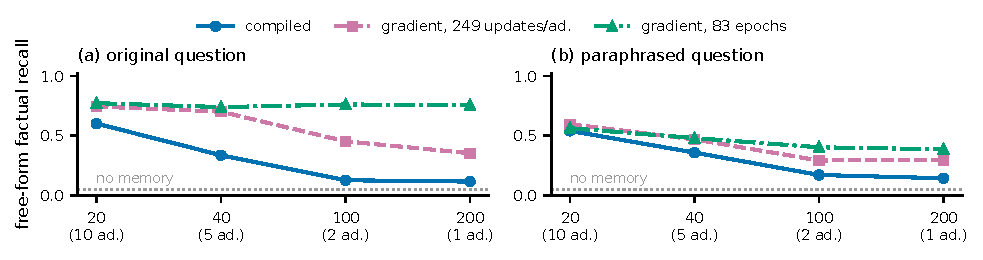
\includegraphics[width=\linewidth]{figs/granularity.pdf}
  \\[4pt]
  {\footnotesize\setlength{\tabcolsep}{4pt}
\begin{tabular}{rrrrrrrrrrr}
\toprule
& & \multicolumn{2}{c}{compiled} & \multicolumn{2}{c}{gradient, 249 updates} & \multicolumn{3}{c}{gradient, 83 epochs} & \multicolumn{2}{c}{bank} \\
\cmidrule(lr){3-4}\cmidrule(lr){5-6}\cmidrule(lr){7-9}\cmidrule(lr){10-11}
facts/ad. & ad. & orig. & para. & orig. & para. & orig. & para. & upd. & MB & comp.\ build s \\
\midrule
20 & 10 & 0.602 & 0.541 & 0.746 & 0.597 & 0.773 & 0.564 & 249 & 283.2 & 7.06 \\
40 & 5 & 0.337 & 0.359 & 0.702 & 0.470 & 0.740 & 0.481 & 415 & 141.6 & 3.80 \\
100 & 2 & 0.127 & 0.171 & 0.453 & 0.293 & 0.762 & 0.403 & 1079 & 56.6 & 1.74 \\
200 & 1 & 0.116 & 0.144 & 0.354 & 0.298 & 0.757 & 0.387 & 2075 & 28.3 & 1.14 \\
\midrule
\multicolumn{2}{r}{\itshape $20\to200$, $p$} & $1.4\mathrm{e}{-23}$ & $5.2\mathrm{e}{-19}$ & $8.4\mathrm{e}{-17}$ & $9.0\mathrm{e}{-11}$ & 0.77 & $2.1\mathrm{e}{-5}$ & & & \\
\bottomrule
\end{tabular}
}
  \caption{\textbf{Granularity depends on the construction regime.} The $x$ axis
  is facts per adapter over one fixed \NPerArm{}-fact memory, per-adapter rank
  held at 16 and \ResidentMB{}\,MB, built three ways; oracle-routed,
  $n=\CurveNPaired{}$ paired items. (a) On original questions the compiled and
  fixed-update regimes decline as partitions coarsen while the equal-exposure
  regime does not; (b) on paraphrased questions all three degrade. Bank build
  seconds are for the compiled regime; the table's last row is the end-to-end
  $20\to\NPerArm{}$ paired test in each regime.}
  \label{fig:granularity}
\end{figure}

\paragraph{Compiled adapters.} Recall falls from \GTwentyQ{} at 20 facts per
adapter to \GTwoHundredQ{} at \NPerArm{}, against a base rate of \BaseQ{}: the
steepest granularity dependence of the three regimes, front-loaded, with 100 to
\NPerArm{} unresolved ($p=\StepHundredtoTwoHundredP{}$). That floor is a property
of the compiled generator at this rank and budget, not of adapters in general:
the gradient regimes reach higher recall at the same partition sizes and rank.

\paragraph{Gradient adapters at a fixed update budget.} Giving every adapter
exactly \SeedSteps{} optimizer updates reproduces the decline, \SeedGTwentyQ{} to
\SeedGTwoHundredQ{}, with \SeedCurveLost{} items lost and \SeedCurveGained{}
gained end to end ($p=\SeedCurveP{}$). This budget is per adapter, not across the
bank, since finer partitions contain more adapters; under it, finer partitions
substantially improve factual recall.

\paragraph{Gradient adapters at equal per-fact exposure.} Holding exposure rather
than updates fixed, original-question recall remains \ExpQLo{}--\ExpQHi{} across
the tested granularities, none of the three paired comparisons against 20 facts
per adapter reaching significance (all $p\ge\ExpQPMin{}$): the monotonic
original-question decline is not observed here. That is an unresolved comparison,
not evidence of equivalence, which would require an equivalence test we did not
perform; and coarser adapters reach it only by taking up to
\ExpGTwoHundredSteps{} updates against \ExpGTwentySteps{}.

\paragraph{Robustness behaves differently.} The paraphrase penalty does not
dissolve under equal exposure: recall on paraphrased questions still falls from
\ExpGTwentyPQ{} to \ExpGTwoHundredPQ{} (\ExpCurvePQLost{} lost,
\ExpCurvePQGained{} gained, $p=\ExpCurvePQP{}$), and the same comparison is
resolved in the fixed-update and compiled regimes (Figure~\ref{fig:granularity}).
Whatever extra exposure supplies to a coarse partition, it restores original
phrasing more readily than robustness to rephrasing.

\paragraph{Direct interaction and author clustering.} The equal-exposure
dissociation is also resolved directly: the 20-to-200 coarsening penalty is
\ExpInteraction{} larger for paraphrased than original questions. An
author-clustered bootstrap over the \NAuthorClusters{} authors gives a 95\%
interval of [\ExpInteractionCILo{}, \ExpInteractionCIHi{}] (exact author-level
sign-flip $p=\ExpInteractionP{}$). Author-level endpoint tests preserve the
other central readings: compiled and fixed-update original recall decline
($p=0.002$ each), equal-exposure original recall does not ($p=0.719$), and its
paraphrase recall declines ($p=0.008$). We retain item-level tests for this
evaluated memory and use the author analysis as a clustered sensitivity check.

\subsection{What finer partitioning costs}
\label{sec:cost}

At fixed \ResidentMB{}\,MB per adapter, finer partitioning raises total bank
storage from \GTwoHundredTotMB{}\,MB to \GTwentyTotMB{}\,MB
(\StorageRatio{}$\times$ for the identical \NPerArm{} facts) and compiled
construction from \GTwoHundredBuild{}\,s to \GTwentyBuild{}\,s
(Figure~\ref{fig:granularity}). Two serving-time costs stay flat: resident memory,
since one partition is active per query, and prompt length, since the selected
memory arrives as weights.

Gradient construction follows the resource constraint: fixed-update bank time
falls from \SeedBuildTwenty{}\,s at 20 facts per adapter to
\SeedBuildTwoHundred{}\,s at 200 as the bank shrinks from ten adapters to one.
Under 83 equal-exposure epochs, bank time stays near
\ExpBuildHundred{}--\ExpBuildTwoHundred{}\,s across granularities because the
bank processes roughly the same total number of records.

The third cost is routing, and it can be wrong. Our lexical router reaches
\RouterTopOne{} top-1 accuracy at 20 facts per adapter, misrouting
\RouterMisGTwenty{} of \NPerArm{} items, but we claim no headline routing tax:
oracle-versus-predicted differences are at most \MaxRoutingDelta{} absolute, below
the engine's reproducibility floor. Multi-LoRA decoding under concurrency is not
bitwise reproducible at temperature zero here; repeating the coarsest arm changed
\NondetGens{} generations and \NondetChanged{} graded outcome.

\subsection{Operating points: in-context and parametric memory}
\label{sec:operating}

Table~\ref{tab:operating} compares memory organizations on the same items at the
same 4B scale; none wins everywhere.

\begin{table}[t]
  \centering
  \caption{Operating points for the same \NPerArm{}-fact memory. Prompt tokens
  recur per query, as a ratio to the \ParamTokens{}-token parametric prompt;
  bank MB and bank build seconds are one-time totals across the ten-adapter g20
  bank (the text gives per-adapter build seconds), and zero means no
  adapter-construction cost, not zero indexing or serving infrastructure.}
  \label{tab:operating}
  \small
  \setlength{\tabcolsep}{4.5pt}
\begin{tabular}{lrrrrr}
\toprule
memory organization & orig.\ q & para.\ q & prompt tok. & bank MB & bank build s \\
\midrule
Base (no memory) & 0.050 & 0.072 & 1$\times$ & 0 & 0 \\
Full context (all \NPerArm{} facts) & 0.862 & 0.834 & 131.4$\times$ & 0 & 0 \\
Top-5 retrieval & 0.729 & 0.613 & 4.67$\times$ & 0 & 0 \\
Compiled, 20 f/ad. & 0.602 & 0.541 & 1$\times$ & 283.2 & 7.06 \\
Gradient, 20 f/ad. & 0.779 & 0.597 & 1$\times$ & 283.2 & 1731.5 \\
\bottomrule
\end{tabular}

\end{table}

\textbf{Full context.} At this corpus size all \NPerArm{} facts fit directly in
context, the highest recall among these five points, \FullCtxQ{}
original and \FullCtxPQ{} paraphrased (\FullCtxNHit{}\,/\,\FullCtxNGrad{} correct,
Wilson 95\% CI [\FullCtxQCILo{}, \FullCtxQCIHi{}]), with no resolved paraphrase
penalty (\FullCtxLost{} lost, \FullCtxGained{} gained, $p=\FullCtxRetP{}$). It
uses \FullCtxTokens{} prompt tokens per query, \FullCtxRatio{}$\times$ the
parametric prompt and \FullCtxRatioRetr{}$\times$ top-5 retrieval; these are
prompt-token measurements, and we infer no latency or throughput ratios from them.
Since this arm answers the same items with the same grader, questions and grader
alone do not account for the parametric paraphrase decline, though storage is not
established as its sole mechanism.

\textbf{Top-5 retrieval} is intermediate on both axes, \RetrQ{} original recall at
\PromptTokenRatio{}$\times$ the parametric prompt, with zero adapter cost in our
accounting: not a claim that retrieval is free, since it needs an index, a scorer,
and the corpus.

\textbf{Gradient-trained adapters} at 20-fact granularity reach the highest
original-question recall among the matched parametric points (\SgdQ{}), but take
\SgdBuildPer{}\,s per adapter to build against \DtwoLBuildPer{}\,s
compiled; trained on all \NPerArm{} facts at once with a wider target-module set
they reach \SgdFullQ{} but fall to \SgdFullPQ{} under paraphrase.
\textbf{Compiled adapters} are below both on raw recall and \BuildRatio{}$\times$
cheaper to construct here.

Figure~\ref{fig:granularity} and Table~\ref{tab:operating} use independently
trained 20-fact gradient banks. The figure's seed-controlled bank was rebuilt
jointly for the granularity ladder and scores \SeedGTwentyQ{}; the table retains
the earlier step-matched bank built for routing and systems accounting, scoring
\SgdQ{}. Both use rank 16, \texttt{down\_proj}, and 249 updates, but they are
different adapter artifacts and evaluation passes.

\textbf{Paraphrase robustness} we report within each arm, not as a ranking.
Rewording costs the gradient arm significantly (retention \SgdRet{},
$p=\SgdRetP{}$) and the top-5 retrieval arm significantly (\RetrRet{},
$p=\RetrRetP{}$), while neither the compiled arm's drop (\GTwentyRet{},
$p=\GTwentyRetP{}$) nor the full-context arm's (\FullCtxRet{},
$p=\FullCtxRetP{}$) is resolvable at this sample size. On a common-correct paired
test every pairwise comparison between the parametric and top-5 retrieval arms is
non-significant (all $p\ge\PairMinP{}$), so we do not rank them here. As a control,
on questions unrelated to the stored facts all arms sit near the floor (base
\NearBase{}, compiled \NearGTwenty{}, retrieval \NearRetr{}).

\subsection{Reliability of parametric memory in serving}
\label{sec:reliability}

A successful adapter load is not evidence that the intended parametric memory is
active: in vLLM 0.24.0 an adapter with mismatched tensor names loads with HTTP
200 while applying \emph{zero} weights, flattening the curve toward the base
rate, a silent failure indistinguishable from a negative result. Treating
bitwise-identical logprobs as failure, every evaluated parametric adapter passed
a log-probability activity gate against a base-versus-base noise floor.

\section{Limitations}
\label{sec:limits}

\paragraph{Routing is easy here.} TOFU names the author in the question, so
selecting the partition is close to a keyword match, whereas real personal memory
refers to entities obliquely and has overlapping partitions. Our routing numbers
are an upper bound and the tax unresolved, not zero.

\paragraph{One dataset, one scale, one adapter configuration.} A single 4B base,
one target-module set, rank 16, one learning rate, and for the compiled arm one
compiler. We did not sweep adapter capacity, so we make no claim about how these
curves move with rank, and prior work indicates the saturation point does
move~\citep{loramem}. TOFU is fictitious and biographical; we rely on the base arm
rather than a non-exposure guarantee, and its paraphrases are human rewrites, not
natural queries.

\paragraph{Facts and entities co-vary.} Partitions are author-aligned, so 20,
40, 100, and 200 facts also mean 1, 2, 5, and 10 authors per adapter. The
coarse-partition penalty may therefore include entity-binding or cross-entity
interference, not only the number of stored records.

\paragraph{The construction budget is part of the result.} Optimizer budget and
exposure materially change the relationship between granularity and
original-question recall, so a granularity sweep does not measure adapter capacity
on its own and we do not report one as if it did. We tested two points in that
space, not the space itself; intermediate budgets, schedules, and optimizers are
unmeasured, and the equal-exposure conditions also differ in scheduler horizon,
which we did not separate from exposure. We control initialization within the
fixed-update ladder but do not estimate variance across independent training
seeds. The independently trained 20-fact banks differ by 0.033, underscoring that
run-level variance is unmeasured.

\paragraph{Our comparison is not a general verdict on in-context memory.} We
charge top-5 retrieval for prompt tokens, not its index, corpus, or retriever
infrastructure, and prompt-token ratios do not establish latency or throughput
under load. At \NPerArm{} facts the whole memory fits in a 16k context and performs
best; we did not vary corpus scale, so we do not identify where full context becomes
inferior or infeasible, and \citet{dataquality} reports the opposite ordering on a
15-document corpus. Our full-context prompts used a fixed order, confounding
position with item difficulty. Finally, we measure factual recall, not what
an adapter carries \emph{well}: TOFU holds voice constant, a clean fact and
unusable style benchmark.

\paragraph{Compiler scope.} All compiled documents were consumed without
truncation, but the coarse documents are longer than the compiler's
meta-training chunks. The compiled curve can therefore reflect both adapter
granularity and compiler distribution shift; the gradient regimes provide a
second construction mechanism but do not identify which explains the compiled
arm's steeper decline.

\section{Conclusion}

Personal memory can be supplied as prompt tokens or encoded in adapter weights,
with different selection requirements and operating costs. Among the five matched
operating points, placing the whole memory in context reaches \FullCtxQ{} original
and \FullCtxPQ{} paraphrased recall at \FullCtxRatio{}$\times$ the parametric
prompt tokens per query under this prompting policy. Among parametric
organizations, fine partitioning helps when construction updates are constrained
and aids robustness to rewording in every regime, but under equal per-fact
exposure the monotonic original-question decline is not observed. Which
organization fits depends on the constrained resource, not on adapter capacity
alone.

\bibliographystyle{plainnat}
\bibliography{refs}

% The checklist follows the references and is not counted against the seven-page
% body limit.
\newpage
\section*{NeurIPS Paper Checklist}
% NeurIPS 2026 paper checklist.
%
% Kept in a SEPARATE file on purpose. The camera-ready workshop limit is seven
% content pages
% against the body only; the checklist is submitted alongside and must not be
% allowed to push the body over. Compile standalone with build_checklist.sh, or
% \input it after \bibliography when the venue asks for a single file.
%
% Every answer below points at the section that actually contains the evidence.
% "Yes" is used only where the PAPER reports the thing, not where we merely
% could have. Where evidence exists only in artifacts or code and not in the
% manuscript, that is stated explicitly in the justification.

\begin{enumerate}

\item {\bf Claims}
    \item[] Question: Do the main claims made in the abstract and introduction
    accurately reflect the paper's contributions and scope?
    \item[] Answer: \answerYes{}
    \item[] Justification: The abstract and the three contribution bullets
    (\S\ref{sec:intro}) each name the measurement that backs them: the
    granularity sweep in three adapter-construction regimes
    (\S\ref{sec:curve}), the storage/construction/routing accounting
    (\S\ref{sec:cost}), and the five-way operating-point comparison including
    full context and top-5 retrieval (\S\ref{sec:operating}). Scope is stated in
    the same sentences: one 4B model, one \NPerArm{}-fact TOFU memory,
    per-adapter rank fixed at 16. Where the abstract says the monotonic
    original-question decline is not observed under equal per-fact exposure, the
    text states that this is an unresolved comparison rather than an equivalence
    result (\S\ref{sec:curve}). The abstract closes by declining to name a
    winner, which matches \S\ref{sec:operating}.

\item {\bf Limitations}
    \item[] Question: Does the paper discuss the limitations of the work
    performed by the authors?
    \item[] Answer: \answerYes{}
    \item[] Justification: \S\ref{sec:limits} is four dedicated paragraphs:
    routing is unusually easy on TOFU and our routing numbers are an upper
    bound; a single base model, target-module set, rank and learning rate, with
    no capacity sweep, so no claim about how these curves move with rank; the
    construction budget is part of the result, so a granularity sweep does not
    measure adapter capacity on its own and we tested two points in the
    budget/exposure space rather than the space itself, with scheduler horizon
    not separated from exposure in the equal-exposure arm; and the in-context
    comparison charges top-5 retrieval for prompt tokens but not for index,
    corpus, or retriever infrastructure, does not vary corpus scale (citing a
    paper that reports the opposite ordering at a smaller corpus), used one
    fixed full-context ordering so position is confounded with item difficulty,
    and measures factual recall only, since TOFU holds authorial voice constant.
    The routing tax is explicitly reported as unresolved rather than zero,
    because it falls below the engine's own reproducibility floor
    (\S\ref{sec:cost}).

\item {\bf Theory assumptions and proofs}
    \item[] Question: For each theoretical result, does the paper provide the
    full set of assumptions and a complete (and correct) proof?
    \item[] Answer: \answerNA{}
    \item[] Justification: The paper is purely empirical. It states no theorem
    and derives no analytical result.

\item {\bf Experimental result reproducibility}
    \item[] Question: Does the paper fully disclose all the information needed
    to reproduce the main experimental results?
    \item[] Answer: \answerYes{}
    \item[] Justification: \S\ref{sec:design} gives the dataset and exact config
    (TOFU \texttt{forget10\_perturbed}), the partition rule (author-aligned
    20-fact blocks packed in ascending order, which is deterministic), the base
    model, rank, learning rate, $\alpha$, target module, optimizer, batch size
    and gradient accumulation, the grading rule and threshold, the pairing and
    test procedure, and the serving stack with versions. Both gradient
    construction regimes are specified separately: the fixed-update regime
    (exactly \SeedSteps{} optimizer updates per adapter, RNGs reset to seed
    \SeedSeed{} immediately before LoRA initialization, termination verified by
    reading \texttt{global\_step} back) and the equal-exposure regime
    (\ExpEpochs{} epochs per partition, trained independently each with its own
    scheduler horizon, giving \ExpGTwentySteps{}--\ExpGTwoHundredSteps{}
    updates). Two controls needed to reproduce the result honestly are also
    described: the per-document truncation gate (\S\ref{sec:design}) and the
    log-probability activity gate (\S\ref{sec:reliability}). Caveats stated in
    the paper: the serving stack is not bitwise reproducible under concurrency
    (\S\ref{sec:cost}), so exact per-item replication is not expected, and the
    full-context arm required a server configured with a 16{,}384-token context
    window rather than the configuration used by the other arms.

\item {\bf Open access to data and code}
    \item[] Question: Does the paper provide open access to the data and code?
    \item[] Answer: \answerYes{}
    \item[] Justification: The camera-ready release includes the experiment
    scripts, frozen per-item results, generated tables and figures, environment
    details, and step-by-step reproduction instructions. The public TOFU
    dataset and Qwen base model are cited at their points of use.

\item {\bf Experimental setting/details}
    \item[] Question: Does the paper specify all the training and test details
    needed to understand the results?
    \item[] Answer: \answerYes{}
    \item[] Justification: \S\ref{sec:design} specifies rank 16, the MLP-side
    target module (\texttt{down\_proj}), the learning rate ($\LearningRate{}$)
    and $\alpha$ (\LoraAlpha{}) held constant across the ladder, the oracle and
    predicted routing procedures, the grading threshold of 0.7, and
    $n=\NGradable{}$ of \NPerArm{} after dropping ungradable items pairwise. The
    two granularity regimes are distinguished explicitly, since optimizer
    updates and per-fact exposure cannot both be held fixed while partition size
    varies: fixed-update (\SeedSteps{} updates per adapter) and equal-exposure
    (\ExpEpochs{} epochs per partition). The operating-point comparison of
    \S\ref{sec:operating} uses a separate step-matched gradient arm
    (\SgdOptSteps{} steps per adapter), and the paper states that its numbers
    are not interchangeable with the granularity regimes.

\item {\bf Experiment statistical significance}
    \item[] Question: Does the paper report error bars suitably and correctly
    defined or other appropriate information about the statistical significance
    of the experiments?
    \item[] Answer: \answerYes{}
    \item[] Justification: Because the same \NPerArm{} items recur at every
    point on the ladder, comparisons are paired at the item level and tested
    with exact McNemar on discordant pairs. The end-to-end $20\to\NPerArm{}$
    paired $p$-value is reported for each of the three construction regimes, on
    both original and paraphrased questions, in the table inside
    Figure~\ref{fig:granularity}, and lost/gained counts are given in the text
    (\S\ref{sec:design}, \S\ref{sec:curve}). Interval types are distinguished:
    granularity-curve aggregate intervals use an item-clustered bootstrap that
    resamples items and carries all of an item's measurements together, whereas
    single-arm binomial intervals, including the full-context 95\% interval in
    \S\ref{sec:operating}, are Wilson intervals.
    Figure~\ref{fig:granularity} plots point estimates
    without error bars, with significance carried by the paired tests in the
    accompanying table rather than by interval overlap. The paper also states
    where a difference is \emph{not} resolvable rather than reporting it as an
    effect: the 100-to-\NPerArm{} compiled step
    ($p=\StepHundredtoTwoHundredP{}$), every equal-exposure original-question
    comparison against 20 facts per adapter (all $p\ge\ExpQPMin{}$, described as
    unresolved rather than as equivalence), and the routing tax, which sits
    below the engine's reproducibility floor.

\item {\bf Experiments compute resources}
    \item[] Question: Does the paper provide sufficient information on the
    computer resources needed to reproduce the experiments?
    \item[] Answer: \answerYes{}
    \item[] Justification: \S\ref{sec:design} states one MI300X GPU running vLLM
    0.24.0 on ROCm 7.2.3 with a 4B base model. Construction cost, which is the
    dominant compute term and is itself a reported result, is given per adapter
    in the prose of \S\ref{sec:operating} (\DtwoLBuildPer{}\,s compiled against
    \SgdBuildPer{}\,s gradient-trained), whereas Table~\ref{tab:operating}
    reports the corresponding ten-adapter bank totals (\GTwentyBuild{}\,s
    compiled against \SgdBuildTotal{}\,s gradient-trained); per-granularity
    compiled build seconds appear in the table
    inside Figure~\ref{fig:granularity}. Evaluation cost is not separately
    tabulated, and we report prompt tokens rather than wall-clock time for the
    in-context arms, since the full-context arm ran under a different server
    configuration and its runtime is not comparable to the others.

\item {\bf Code of ethics}
    \item[] Question: Does the research conducted in the paper conform, in every
    respect, with the NeurIPS Code of Ethics?
    \item[] Answer: \answerYes{}
    \item[] Justification: The study uses a public synthetic benchmark of
    fictitious author biographies and a public base model. No human subjects, no
    personal or private data, and no annotator labour are involved.

\item {\bf Broader impacts}
    \item[] Question: Does the paper discuss both potential positive societal
    impacts and negative societal impacts of the work performed?
    \item[] Answer: \answerNA{}
    \item[] Justification: The work is a measurement study of where a personal
    agent should store facts. It introduces no new model, capability, or
    artifact for release. We note that the setting concerns private user data,
    but our results are about how finely a memory is partitioned and how the
    adapters are constructed, not about whether stored information can be
    recovered or removed; the paper makes no privacy or unlearning claim, and we
    do not consider the measurement itself to carry a distinct societal risk.

\item {\bf Safeguards}
    \item[] Question: Does the paper describe safeguards that have been put in
    place for responsible release of data or models that have a high risk for
    misuse?
    \item[] Answer: \answerNA{}
    \item[] Justification: No data, model, or scraped corpus is released with
    this submission, and the adapters trained here encode only fictitious
    biographies from a public benchmark, so there is no misuse surface to guard.

\item {\bf Licenses for existing assets}
    \item[] Question: Are the creators or original owners of assets used in the
    paper properly credited and are the license and terms of use explicitly
    mentioned and properly respected?
    \item[] Answer: \answerYes{}
    \item[] Justification: Every asset used is cited at the point of use in
    \S\ref{sec:design}: TOFU~\citep{tofu} for the data, Qwen3-4B-Instruct-2507
    base~\citep{qwen3,qwen3-4b-2507} for the model, the document-to-LoRA
    hypernetwork~\citep{d2l} for the compiled generator, LoRA~\citep{lora} for
    the gradient arm, and retrieval-augmented generation~\citep{rag} for the
    retrieval arm. Note honestly: individual license names and versions are not
    printed in the manuscript; all assets used are publicly released and used
    within their published terms, and license details will accompany the code
    release.

\item {\bf New assets}
    \item[] Question: Are new assets introduced in the paper well documented and
    is the documentation provided alongside the assets?
    \item[] Answer: \answerNA{}
    \item[] Justification: This submission releases no new asset. The adapters
    built for the study are experimental artifacts, not a contributed model.

\item {\bf Crowdsourcing and research with human subjects}
    \item[] Question: For crowdsourcing experiments and research with human
    subjects, does the paper include the full text of instructions given to
    participants and screenshots, if applicable, as well as details about
    compensation?
    \item[] Answer: \answerNA{}
    \item[] Justification: No crowdsourcing and no human subjects. The
    paraphrases used in the evaluation are the human-written paraphrases shipped
    with the TOFU benchmark, not collected by us.

\item {\bf Institutional review board (IRB) approvals or equivalent for research
with human subjects}
    \item[] Question: Does the paper describe potential risks incurred by study
    participants, whether such risks were disclosed to the subjects, and whether
    Institutional Review Board (IRB) approvals (or an equivalent approval/review
    based on the requirements of your country or institution) were obtained?
    \item[] Answer: \answerNA{}
    \item[] Justification: No study participants and no human-subjects research,
    so no review was required.

\item {\bf Declaration of LLM usage}
    \item[] Question: Does the paper describe the usage of LLMs if it is an
    important, original, or non-standard component of the core methods in this
    research?
    \item[] Answer: \answerYes{}
    \item[] Justification: Language models are the object of study, and every
    such use is described in \S\ref{sec:design}: a Qwen3-4B-Instruct-2507 base as the
    model under test, a document-to-LoRA hypernetwork as the compiled-memory
    generator, gradient-trained LoRA for the gradient arm, and the same base
    prompted with
    retrieved or full-corpus context for the in-context arms. Grading is a
    deterministic token-recall rule against the gold answer, not an LLM judge.

\end{enumerate}


\end{document}
